\documentclass[twoside]{book}

% Packages required by doxygen
\usepackage{fixltx2e}
\usepackage{calc}
\usepackage{doxygen}
\usepackage[export]{adjustbox} % also loads graphicx
\usepackage{graphicx}
\usepackage[utf8]{inputenc}
\usepackage{makeidx}
\usepackage{multicol}
\usepackage{multirow}
\PassOptionsToPackage{warn}{textcomp}
\usepackage{textcomp}
\usepackage[nointegrals]{wasysym}
\usepackage[table]{xcolor}

% Font selection
\usepackage[T1]{fontenc}
\usepackage[scaled=.90]{helvet}
\usepackage{courier}
\usepackage{amssymb}
\usepackage{sectsty}
\renewcommand{\familydefault}{\sfdefault}
\allsectionsfont{%
  \fontseries{bc}\selectfont%
  \color{darkgray}%
}
\renewcommand{\DoxyLabelFont}{%
  \fontseries{bc}\selectfont%
  \color{darkgray}%
}
\newcommand{\+}{\discretionary{\mbox{\scriptsize$\hookleftarrow$}}{}{}}

% Page & text layout
\usepackage{geometry}
\geometry{%
  a4paper,%
  top=2.5cm,%
  bottom=2.5cm,%
  left=2.5cm,%
  right=2.5cm%
}
\tolerance=750
\hfuzz=15pt
\hbadness=750
\setlength{\emergencystretch}{15pt}
\setlength{\parindent}{0cm}
\setlength{\parskip}{3ex plus 2ex minus 2ex}
\makeatletter
\renewcommand{\paragraph}{%
  \@startsection{paragraph}{4}{0ex}{-1.0ex}{1.0ex}{%
    \normalfont\normalsize\bfseries\SS@parafont%
  }%
}
\renewcommand{\subparagraph}{%
  \@startsection{subparagraph}{5}{0ex}{-1.0ex}{1.0ex}{%
    \normalfont\normalsize\bfseries\SS@subparafont%
  }%
}
\makeatother

% Headers & footers
\usepackage{fancyhdr}
\pagestyle{fancyplain}
\fancyhead[LE]{\fancyplain{}{\bfseries\thepage}}
\fancyhead[CE]{\fancyplain{}{}}
\fancyhead[RE]{\fancyplain{}{\bfseries\leftmark}}
\fancyhead[LO]{\fancyplain{}{\bfseries\rightmark}}
\fancyhead[CO]{\fancyplain{}{}}
\fancyhead[RO]{\fancyplain{}{\bfseries\thepage}}
\fancyfoot[LE]{\fancyplain{}{}}
\fancyfoot[CE]{\fancyplain{}{}}
\fancyfoot[RE]{\fancyplain{}{\bfseries\scriptsize Generated by Doxygen }}
\fancyfoot[LO]{\fancyplain{}{\bfseries\scriptsize Generated by Doxygen }}
\fancyfoot[CO]{\fancyplain{}{}}
\fancyfoot[RO]{\fancyplain{}{}}
\renewcommand{\footrulewidth}{0.4pt}
\renewcommand{\chaptermark}[1]{%
  \markboth{#1}{}%
}
\renewcommand{\sectionmark}[1]{%
  \markright{\thesection\ #1}%
}

% Indices & bibliography
\usepackage{natbib}
\usepackage[titles]{tocloft}
\setcounter{tocdepth}{3}
\setcounter{secnumdepth}{5}
\makeindex

% Hyperlinks (required, but should be loaded last)
\usepackage{ifpdf}
\ifpdf
  \usepackage[pdftex,pagebackref=true]{hyperref}
\else
  \usepackage[ps2pdf,pagebackref=true]{hyperref}
\fi
\hypersetup{%
  colorlinks=true,%
  linkcolor=blue,%
  citecolor=blue,%
  unicode%
}

% Custom commands
\newcommand{\clearemptydoublepage}{%
  \newpage{\pagestyle{empty}\cleardoublepage}%
}

\usepackage{caption}
\captionsetup{labelsep=space,justification=centering,font={bf},singlelinecheck=off,skip=4pt,position=top}

%===== C O N T E N T S =====

\begin{document}

% Titlepage & ToC
\hypersetup{pageanchor=false,
             bookmarksnumbered=true,
             pdfencoding=unicode
            }
\pagenumbering{alph}
\begin{titlepage}
\vspace*{7cm}
\begin{center}%
{\Large My Project }\\
\vspace*{1cm}
{\large Generated by Doxygen 1.8.13}\\
\end{center}
\end{titlepage}
\clearemptydoublepage
\pagenumbering{roman}
\tableofcontents
\clearemptydoublepage
\pagenumbering{arabic}
\hypersetup{pageanchor=true}

%--- Begin generated contents ---
\chapter{Main Page}
\label{index}\hypertarget{index}{}This is the main file of the program. This will be used to launch the interface to select files and other things. Refer to class list for detailed description of other classes. 
\chapter{Hierarchical Index}
\section{Class Hierarchy}
This inheritance list is sorted roughly, but not completely, alphabetically\+:\begin{DoxyCompactList}
\item \contentsline{section}{Edge}{\pageref{structEdge}}{}
\item \contentsline{section}{Edge\+Loop}{\pageref{classEdgeLoop}}{}
\item \contentsline{section}{Fig3D}{\pageref{classFig3D}}{}
\item \contentsline{section}{partial\+Order}{\pageref{classpartialOrder}}{}
\item \contentsline{section}{Plane}{\pageref{structPlane}}{}
\item Q\+Main\+Window\begin{DoxyCompactList}
\item \contentsline{section}{Main\+Window}{\pageref{classMainWindow}}{}
\item \contentsline{section}{option\+Window}{\pageref{classoptionWindow}}{}
\end{DoxyCompactList}
\item \contentsline{section}{Vertice}{\pageref{structVertice}}{}
\item \contentsline{section}{Wire\+Frame}{\pageref{classWireFrame}}{}
\end{DoxyCompactList}

\chapter{Class Index}
\section{Class List}
Here are the classes, structs, unions and interfaces with brief descriptions\+:\begin{DoxyCompactList}
\item\contentsline{section}{\hyperlink{classEdgeLoop}{Edge\+Loop} }{\pageref{classEdgeLoop}}{}
\item\contentsline{section}{\hyperlink{classpartialOrder}{partial\+Order} }{\pageref{classpartialOrder}}{}
\item\contentsline{section}{\hyperlink{classVertice}{Vertice} }{\pageref{classVertice}}{}
\item\contentsline{section}{\hyperlink{classWireFrame}{Wire\+Frame} }{\pageref{classWireFrame}}{}
\end{DoxyCompactList}

\chapter{File Index}
\section{File List}
Here is a list of all files with brief descriptions\+:\begin{DoxyCompactList}
\item\contentsline{section}{/home/ankurshaswat/\+My\+Files/\+Repos/\+C\+O\+P290/\+Project1/\+Code/include/module1/\hyperlink{Display_8h}{Display.\+h} }{\pageref{Display_8h}}{}
\item\contentsline{section}{/home/ankurshaswat/\+My\+Files/\+Repos/\+C\+O\+P290/\+Project1/\+Code/include/module1/\hyperlink{Edge_8h}{Edge.\+h} }{\pageref{Edge_8h}}{}
\item\contentsline{section}{/home/ankurshaswat/\+My\+Files/\+Repos/\+C\+O\+P290/\+Project1/\+Code/include/module1/\hyperlink{EdgeLoop_8h}{Edge\+Loop.\+h} }{\pageref{EdgeLoop_8h}}{}
\item\contentsline{section}{/home/ankurshaswat/\+My\+Files/\+Repos/\+C\+O\+P290/\+Project1/\+Code/include/module1/\hyperlink{Face_8h}{Face.\+h} }{\pageref{Face_8h}}{}
\item\contentsline{section}{/home/ankurshaswat/\+My\+Files/\+Repos/\+C\+O\+P290/\+Project1/\+Code/include/module1/\hyperlink{Fig2D_8h}{Fig2\+D.\+h} }{\pageref{Fig2D_8h}}{}
\item\contentsline{section}{/home/ankurshaswat/\+My\+Files/\+Repos/\+C\+O\+P290/\+Project1/\+Code/include/module1/\hyperlink{Fig3D_8h}{Fig3\+D.\+h} }{\pageref{Fig3D_8h}}{}
\item\contentsline{section}{/home/ankurshaswat/\+My\+Files/\+Repos/\+C\+O\+P290/\+Project1/\+Code/include/module1/\hyperlink{Vertice_8h}{Vertice.\+h} }{\pageref{Vertice_8h}}{}
\item\contentsline{section}{/home/ankurshaswat/\+My\+Files/\+Repos/\+C\+O\+P290/\+Project1/\+Code/include/module1/\hyperlink{Wireframe_8h}{Wireframe.\+h} }{\pageref{Wireframe_8h}}{}
\item\contentsline{section}{/home/ankurshaswat/\+My\+Files/\+Repos/\+C\+O\+P290/\+Project1/\+Code/src/\hyperlink{program_8cpp}{program.\+cpp} \\*Main file documentation }{\pageref{program_8cpp}}{}
\item\contentsline{section}{/home/ankurshaswat/\+My\+Files/\+Repos/\+C\+O\+P290/\+Project1/\+Code/src/module1/\hyperlink{Fig3D_8cpp}{Fig3\+D.\+cpp} }{\pageref{Fig3D_8cpp}}{}
\end{DoxyCompactList}

\chapter{Class Documentation}
\hypertarget{classEdgeLoop}{}\section{Edge\+Loop Class Reference}
\label{classEdgeLoop}\index{Edge\+Loop@{Edge\+Loop}}


{\ttfamily \#include $<$complex\+Components.\+h$>$}

\subsection*{Public Member Functions}
\begin{DoxyCompactItemize}
\item 
bool \hyperlink{classEdgeLoop_acae6f647805e3f043325f047208556c8}{is\+Contained} (\hyperlink{classEdgeLoop}{Edge\+Loop} a)
\end{DoxyCompactItemize}
\subsection*{Public Attributes}
\begin{DoxyCompactItemize}
\item 
vector$<$ \hyperlink{structVertice}{Vertice} $>$ \hyperlink{classEdgeLoop_a781d9dd73f8b69c7b0075d4297f6b277}{vertices}
\end{DoxyCompactItemize}


\subsection{Detailed Description}
Some high level components used as intermediates in our algorithms a planar closed loop of edges (connected end-\/to-\/end) 

\subsection{Member Function Documentation}
\mbox{\Hypertarget{classEdgeLoop_acae6f647805e3f043325f047208556c8}\label{classEdgeLoop_acae6f647805e3f043325f047208556c8}} 
\index{Edge\+Loop@{Edge\+Loop}!is\+Contained@{is\+Contained}}
\index{is\+Contained@{is\+Contained}!Edge\+Loop@{Edge\+Loop}}
\subsubsection{\texorpdfstring{is\+Contained()}{isContained()}}
{\footnotesize\ttfamily bool Edge\+Loop\+::is\+Contained (\begin{DoxyParamCaption}\item[{\hyperlink{classEdgeLoop}{Edge\+Loop}}]{a }\end{DoxyParamCaption})}

Function to check whether an edge\+Loop is completely contained in another 

\subsection{Member Data Documentation}
\mbox{\Hypertarget{classEdgeLoop_a781d9dd73f8b69c7b0075d4297f6b277}\label{classEdgeLoop_a781d9dd73f8b69c7b0075d4297f6b277}} 
\index{Edge\+Loop@{Edge\+Loop}!vertices@{vertices}}
\index{vertices@{vertices}!Edge\+Loop@{Edge\+Loop}}
\subsubsection{\texorpdfstring{vertices}{vertices}}
{\footnotesize\ttfamily vector$<$\hyperlink{structVertice}{Vertice}$>$ Edge\+Loop\+::vertices}



The documentation for this class was generated from the following file\+:\begin{DoxyCompactItemize}
\item 
/home/ankurshaswat/\+My\+Files/\+Repos/\+C\+O\+P290-\/master/\+E\+D\+\_\+\+Project/include/\hyperlink{complexComponents_8h}{complex\+Components.\+h}\end{DoxyCompactItemize}

\hypertarget{classFace}{}\section{Face Class Reference}
\label{classFace}\index{Face@{Face}}


{\ttfamily \#include $<$Face.\+h$>$}

\subsection*{Public Member Functions}
\begin{DoxyCompactItemize}
\item 
\hyperlink{classEdge}{Edge} $\ast$ \hyperlink{classFace_a5973ddd3395e60aeadc76f24d1bcc860}{get\+Edges} ()
\item 
vector$<$ vector$<$ \hyperlink{classEdge}{Edge} $>$ $>$ \hyperlink{classFace_a3676c176d0ad0b518a74409372aa94da}{planar\+Partitions} ()
\end{DoxyCompactItemize}


\subsection{Member Function Documentation}
\mbox{\Hypertarget{classFace_a5973ddd3395e60aeadc76f24d1bcc860}\label{classFace_a5973ddd3395e60aeadc76f24d1bcc860}} 
\index{Face@{Face}!get\+Edges@{get\+Edges}}
\index{get\+Edges@{get\+Edges}!Face@{Face}}
\subsubsection{\texorpdfstring{get\+Edges()}{getEdges()}}
{\footnotesize\ttfamily \hyperlink{classEdge}{Edge}$\ast$ Face\+::get\+Edges (\begin{DoxyParamCaption}{ }\end{DoxyParamCaption})}

\mbox{\Hypertarget{classFace_a3676c176d0ad0b518a74409372aa94da}\label{classFace_a3676c176d0ad0b518a74409372aa94da}} 
\index{Face@{Face}!planar\+Partitions@{planar\+Partitions}}
\index{planar\+Partitions@{planar\+Partitions}!Face@{Face}}
\subsubsection{\texorpdfstring{planar\+Partitions()}{planarPartitions()}}
{\footnotesize\ttfamily vector$<$ vector$<$\hyperlink{classEdge}{Edge}$>$ $>$ Face\+::planar\+Partitions (\begin{DoxyParamCaption}{ }\end{DoxyParamCaption})}



The documentation for this class was generated from the following files\+:\begin{DoxyCompactItemize}
\item 
/home/ankurshaswat/\+My\+Files/\+Repos/\+C\+O\+P290/\+Project1/\+Code/include/module1/\hyperlink{Face_8h}{Face.\+h}\item 
/home/ankurshaswat/\+My\+Files/\+Repos/\+C\+O\+P290/\+Project1/\+Code/include/module1/\hyperlink{Wireframe_8h}{Wireframe.\+h}\end{DoxyCompactItemize}

\hypertarget{classpartialOrder}{}\section{partial\+Order Class Reference}
\label{classpartialOrder}\index{partial\+Order@{partial\+Order}}


{\ttfamily \#include $<$structs.\+h$>$}



\subsection{Detailed Description}
Custom data structures needed in reconstruction 

The documentation for this class was generated from the following file\+:\begin{DoxyCompactItemize}
\item 
/home/ankurshaswat/\+My\+Files/\+Repos/\+C\+O\+P290/\+Project1/\+Code/include/module1/\hyperlink{structs_8h}{structs.\+h}\end{DoxyCompactItemize}

\hypertarget{classWireFrame}{}\section{Wire\+Frame Class Reference}
\label{classWireFrame}\index{Wire\+Frame@{Wire\+Frame}}


{\ttfamily \#include $<$complex\+Components.\+h$>$}

\subsection*{Public Member Functions}
\begin{DoxyCompactItemize}
\item 
\hyperlink{classWireFrame}{Wire\+Frame} \hyperlink{classWireFrame_a2cbc8d66f5c958499d5ffa3654988d5e}{get\+Transformation} (double Xrot, double Yrot, double Zrot, double Xoff, double Yoff, double Zoff)
\end{DoxyCompactItemize}
\subsection*{Public Attributes}
\begin{DoxyCompactItemize}
\item 
vector$<$ \hyperlink{structEdge}{Edge} $>$ \hyperlink{classWireFrame_a95f1653c5b972aa8514d34c0b7633d75}{edges}
\end{DoxyCompactItemize}


\subsection{Member Function Documentation}
\mbox{\Hypertarget{classWireFrame_a2cbc8d66f5c958499d5ffa3654988d5e}\label{classWireFrame_a2cbc8d66f5c958499d5ffa3654988d5e}} 
\index{Wire\+Frame@{Wire\+Frame}!get\+Transformation@{get\+Transformation}}
\index{get\+Transformation@{get\+Transformation}!Wire\+Frame@{Wire\+Frame}}
\subsubsection{\texorpdfstring{get\+Transformation()}{getTransformation()}}
{\footnotesize\ttfamily \hyperlink{classWireFrame}{Wire\+Frame} Wire\+Frame\+::get\+Transformation (\begin{DoxyParamCaption}\item[{double}]{Xrot,  }\item[{double}]{Yrot,  }\item[{double}]{Zrot,  }\item[{double}]{Xoff,  }\item[{double}]{Yoff,  }\item[{double}]{Zoff }\end{DoxyParamCaption})}

get transformed 3D object 

\subsection{Member Data Documentation}
\mbox{\Hypertarget{classWireFrame_a95f1653c5b972aa8514d34c0b7633d75}\label{classWireFrame_a95f1653c5b972aa8514d34c0b7633d75}} 
\index{Wire\+Frame@{Wire\+Frame}!edges@{edges}}
\index{edges@{edges}!Wire\+Frame@{Wire\+Frame}}
\subsubsection{\texorpdfstring{edges}{edges}}
{\footnotesize\ttfamily vector$<$\hyperlink{structEdge}{Edge}$>$ Wire\+Frame\+::edges}



The documentation for this class was generated from the following files\+:\begin{DoxyCompactItemize}
\item 
/home/ankurshaswat/\+My\+Files/\+Repos/\+C\+O\+P290/working\+\_\+3d\+\_\+to\+\_\+2d/include/module1/\hyperlink{complexComponents_8h}{complex\+Components.\+h}\item 
/home/ankurshaswat/\+My\+Files/\+Repos/\+C\+O\+P290/working\+\_\+3d\+\_\+to\+\_\+2d/src/\hyperlink{complexcomponents_8cpp}{complexcomponents.\+cpp}\end{DoxyCompactItemize}

\chapter{File Documentation}
\hypertarget{basicComponents_8h}{}\section{/home/ankurshaswat/\+My\+Files/\+Repos/\+C\+O\+P290/\+Project1/\+Code/include/module1/basic\+Components.h File Reference}
\label{basicComponents_8h}\index{/home/ankurshaswat/\+My\+Files/\+Repos/\+C\+O\+P290/\+Project1/\+Code/include/module1/basic\+Components.\+h@{/home/ankurshaswat/\+My\+Files/\+Repos/\+C\+O\+P290/\+Project1/\+Code/include/module1/basic\+Components.\+h}}
This graph shows which files directly or indirectly include this file\+:\nopagebreak
\begin{figure}[H]
\begin{center}
\leavevmode
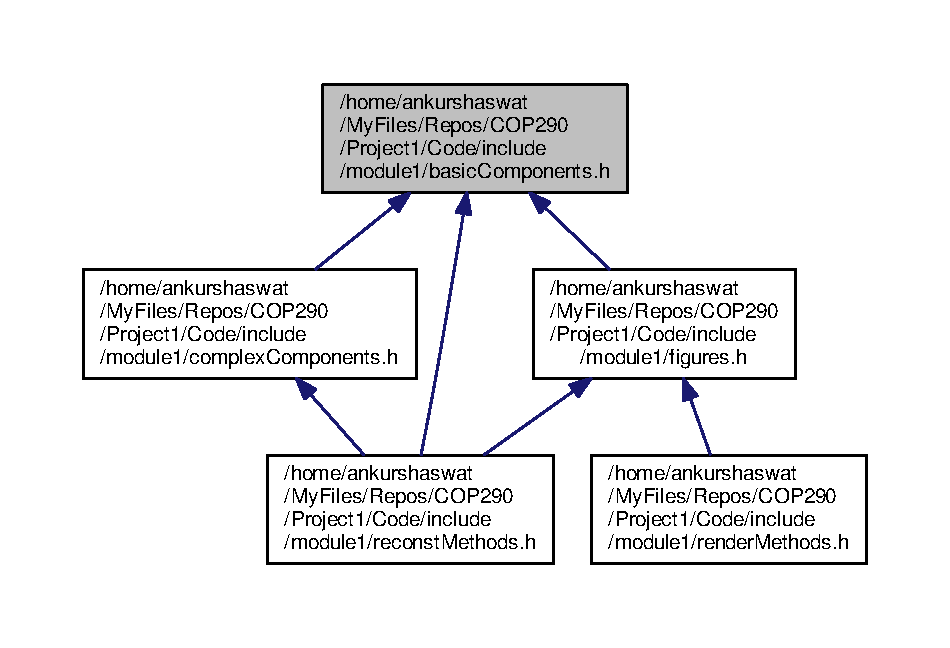
\includegraphics[width=350pt]{basicComponents_8h__dep__incl}
\end{center}
\end{figure}
\subsection*{Classes}
\begin{DoxyCompactItemize}
\item 
class \hyperlink{classVertice}{Vertice}
\end{DoxyCompactItemize}
\subsection*{Variables}
\begin{DoxyCompactItemize}
\item 
class \hyperlink{classVertice}{Vertice} \hyperlink{basicComponents_8h_a9e0e705b8112107f578dafc26a057db1}{edge} \mbox{[}10\mbox{]}
\item 
\hyperlink{classVertice}{Vertice} \hyperlink{basicComponents_8h_a5fb31efa54dedf5bd0e6301985a0af57}{vertice} \mbox{[}10\mbox{]}
\end{DoxyCompactItemize}


\subsection{Variable Documentation}
\mbox{\Hypertarget{basicComponents_8h_a9e0e705b8112107f578dafc26a057db1}\label{basicComponents_8h_a9e0e705b8112107f578dafc26a057db1}} 
\index{basic\+Components.\+h@{basic\+Components.\+h}!edge@{edge}}
\index{edge@{edge}!basic\+Components.\+h@{basic\+Components.\+h}}
\subsubsection{\texorpdfstring{edge}{edge}}
{\footnotesize\ttfamily class \hyperlink{classVertice}{Vertice} edge\mbox{[}10\mbox{]}}

\mbox{\Hypertarget{basicComponents_8h_a5fb31efa54dedf5bd0e6301985a0af57}\label{basicComponents_8h_a5fb31efa54dedf5bd0e6301985a0af57}} 
\index{basic\+Components.\+h@{basic\+Components.\+h}!vertice@{vertice}}
\index{vertice@{vertice}!basic\+Components.\+h@{basic\+Components.\+h}}
\subsubsection{\texorpdfstring{vertice}{vertice}}
{\footnotesize\ttfamily \hyperlink{classVertice}{Vertice} vertice\mbox{[}10\mbox{]}}


\hypertarget{complexComponents_8h}{}\section{/home/ankurshaswat/\+My\+Files/\+Repos/\+C\+O\+P290/\+Project1/\+Code/include/module1/complex\+Components.h File Reference}
\label{complexComponents_8h}\index{/home/ankurshaswat/\+My\+Files/\+Repos/\+C\+O\+P290/\+Project1/\+Code/include/module1/complex\+Components.\+h@{/home/ankurshaswat/\+My\+Files/\+Repos/\+C\+O\+P290/\+Project1/\+Code/include/module1/complex\+Components.\+h}}
{\ttfamily \#include \char`\"{}basic\+Components.\+h\char`\"{}}\newline
Include dependency graph for complex\+Components.\+h\+:\nopagebreak
\begin{figure}[H]
\begin{center}
\leavevmode
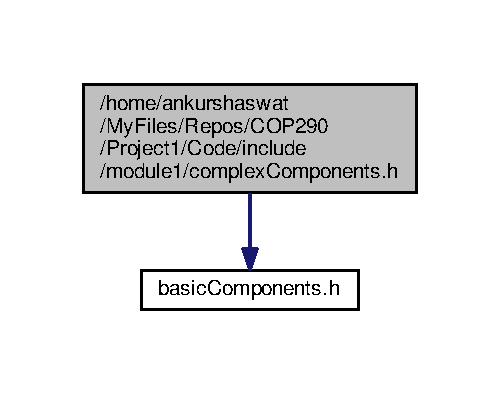
\includegraphics[width=240pt]{complexComponents_8h__incl}
\end{center}
\end{figure}
This graph shows which files directly or indirectly include this file\+:\nopagebreak
\begin{figure}[H]
\begin{center}
\leavevmode
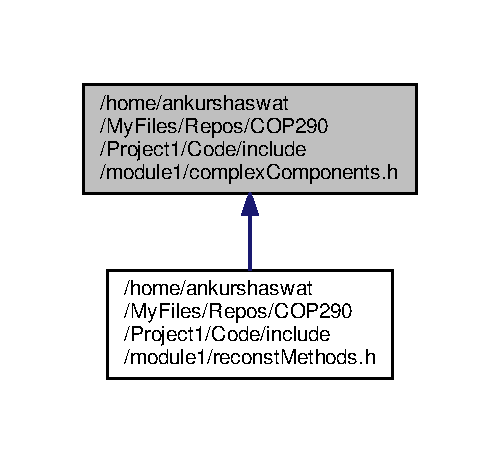
\includegraphics[width=240pt]{complexComponents_8h__dep__incl}
\end{center}
\end{figure}
\subsection*{Classes}
\begin{DoxyCompactItemize}
\item 
class \hyperlink{classEdgeLoop}{Edge\+Loop}
\item 
class \hyperlink{classWireFrame}{Wire\+Frame}
\end{DoxyCompactItemize}

\hypertarget{figures_8h}{}\section{/home/ankurshaswat/\+My\+Files/\+Repos/\+C\+O\+P290/\+Project1/\+Code/include/module1/figures.h File Reference}
\label{figures_8h}\index{/home/ankurshaswat/\+My\+Files/\+Repos/\+C\+O\+P290/\+Project1/\+Code/include/module1/figures.\+h@{/home/ankurshaswat/\+My\+Files/\+Repos/\+C\+O\+P290/\+Project1/\+Code/include/module1/figures.\+h}}
{\ttfamily \#include \char`\"{}basic\+Components.\+h\char`\"{}}\newline
Include dependency graph for figures.\+h\+:
\nopagebreak
\begin{figure}[H]
\begin{center}
\leavevmode
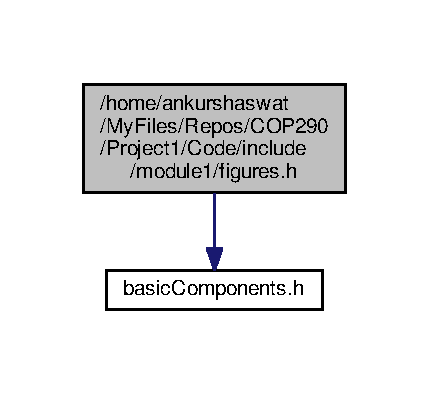
\includegraphics[width=206pt]{figures_8h__incl}
\end{center}
\end{figure}
This graph shows which files directly or indirectly include this file\+:
\nopagebreak
\begin{figure}[H]
\begin{center}
\leavevmode
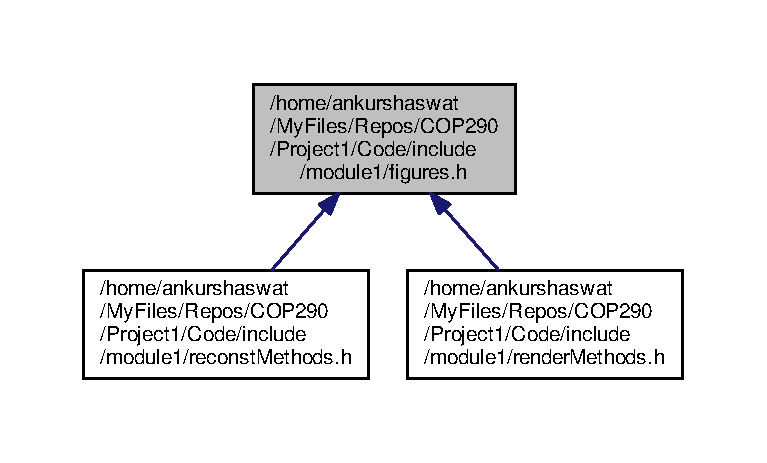
\includegraphics[width=350pt]{figures_8h__dep__incl}
\end{center}
\end{figure}

\hypertarget{reconstMethods_8h}{}\section{/home/ankurshaswat/\+My\+Files/\+Repos/\+C\+O\+P290-\/master/\+E\+D\+\_\+\+Project/include/reconst\+Methods.h File Reference}
\label{reconstMethods_8h}\index{/home/ankurshaswat/\+My\+Files/\+Repos/\+C\+O\+P290-\/master/\+E\+D\+\_\+\+Project/include/reconst\+Methods.\+h@{/home/ankurshaswat/\+My\+Files/\+Repos/\+C\+O\+P290-\/master/\+E\+D\+\_\+\+Project/include/reconst\+Methods.\+h}}
{\ttfamily \#include \char`\"{}basic\+Components.\+h\char`\"{}}\newline
{\ttfamily \#include \char`\"{}complex\+Components.\+h\char`\"{}}\newline
{\ttfamily \#include \char`\"{}figures.\+h\char`\"{}}\newline
{\ttfamily \#include \char`\"{}structs.\+h\char`\"{}}\newline
Include dependency graph for reconst\+Methods.\+h\+:
\nopagebreak
\begin{figure}[H]
\begin{center}
\leavevmode
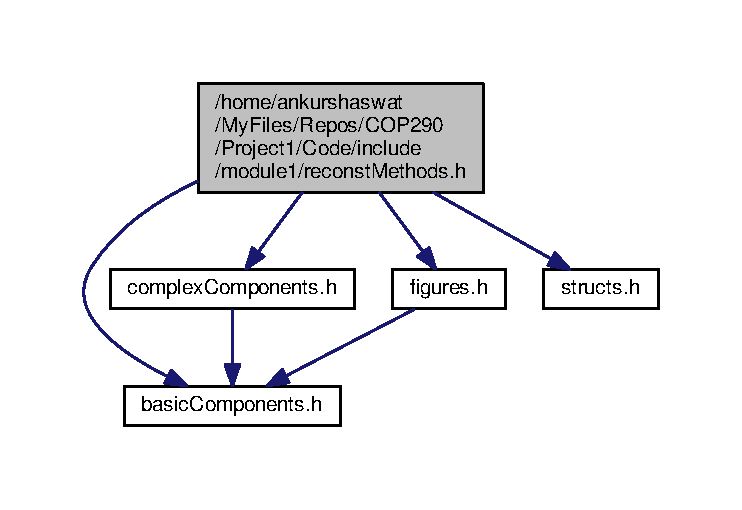
\includegraphics[width=350pt]{reconstMethods_8h__incl}
\end{center}
\end{figure}
This graph shows which files directly or indirectly include this file\+:
\nopagebreak
\begin{figure}[H]
\begin{center}
\leavevmode
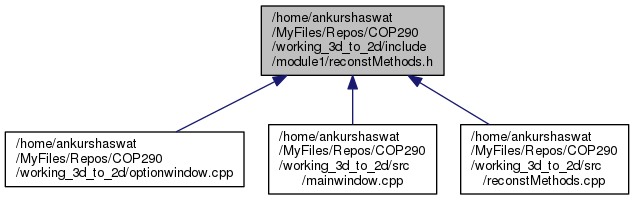
\includegraphics[width=350pt]{reconstMethods_8h__dep__incl}
\end{center}
\end{figure}
\subsection*{Functions}
\begin{DoxyCompactItemize}
\item 
\hyperlink{classWireFrame}{Wire\+Frame} \hyperlink{reconstMethods_8h_a110e71b7da4f490cc73c09b654d2db99}{const\+Uniq3d\+Edges} (vector$<$ vector$<$ \hyperlink{structEdge}{Edge} $>$ $>$ edge\+Set)
\begin{DoxyCompactList}\small\item\em Function to construct 3d edges from 2d edges by checking the possibility of the edges being projections of each other. \end{DoxyCompactList}\item 
std\+::vector$<$ std\+::vector$<$ \hyperlink{structEdge}{Edge} $>$ $>$ \hyperlink{reconstMethods_8h_ab5b36acd93691246a5e348eecc9225cf}{read\+File} (const char $\ast$)
\begin{DoxyCompactList}\small\item\em Function to read txt file contatining labelled data of xy , yz and xz views and returns the result as a vector of vector of edges. \end{DoxyCompactList}\item 
\hyperlink{classFig3D}{Fig3D} \hyperlink{reconstMethods_8h_a323870048d29be8ede27a7020e767c79}{wireframe\+To3D} (\hyperlink{classWireFrame}{Wire\+Frame} a)
\begin{DoxyCompactList}\small\item\em Takes a wireframe object and converts it into a 3d object by creating faces by forming edge loops. \end{DoxyCompactList}\item 
vector$<$ vector$<$ int $>$ $>$ \hyperlink{reconstMethods_8h_ad748b0dac80de637f972c4676f8ccdaa}{coplanar\+Edges} (vector$<$ \hyperlink{structEdge}{Edge} $>$ \&edges)
\item 
vector$<$ vector$<$ int $>$ $>$ \hyperlink{reconstMethods_8h_aed7e2db16ce5e7210f9f80b20a8af52f}{get\+Edge\+Loops} (vector$<$ \hyperlink{structEdge}{Edge} $>$ \&edges, vector$<$ int $>$ coplanar\+Indices)
\end{DoxyCompactItemize}


\subsection{Function Documentation}
\mbox{\Hypertarget{reconstMethods_8h_a110e71b7da4f490cc73c09b654d2db99}\label{reconstMethods_8h_a110e71b7da4f490cc73c09b654d2db99}} 
\index{reconst\+Methods.\+h@{reconst\+Methods.\+h}!const\+Uniq3d\+Edges@{const\+Uniq3d\+Edges}}
\index{const\+Uniq3d\+Edges@{const\+Uniq3d\+Edges}!reconst\+Methods.\+h@{reconst\+Methods.\+h}}
\subsubsection{\texorpdfstring{const\+Uniq3d\+Edges()}{constUniq3dEdges()}}
{\footnotesize\ttfamily \hyperlink{classWireFrame}{Wire\+Frame} const\+Uniq3d\+Edges (\begin{DoxyParamCaption}\item[{vector$<$ vector$<$ \hyperlink{structEdge}{Edge} $>$ $>$}]{edge\+Set }\end{DoxyParamCaption})}



Function to construct 3d edges from 2d edges by checking the possibility of the edges being projections of each other. 

Defines methods required for 3D reconstruction process \mbox{\Hypertarget{reconstMethods_8h_ad748b0dac80de637f972c4676f8ccdaa}\label{reconstMethods_8h_ad748b0dac80de637f972c4676f8ccdaa}} 
\index{reconst\+Methods.\+h@{reconst\+Methods.\+h}!coplanar\+Edges@{coplanar\+Edges}}
\index{coplanar\+Edges@{coplanar\+Edges}!reconst\+Methods.\+h@{reconst\+Methods.\+h}}
\subsubsection{\texorpdfstring{coplanar\+Edges()}{coplanarEdges()}}
{\footnotesize\ttfamily vector$<$ vector$<$int$>$ $>$ coplanar\+Edges (\begin{DoxyParamCaption}\item[{vector$<$ \hyperlink{structEdge}{Edge} $>$ \&}]{edges }\end{DoxyParamCaption})}

Returns coplanar sets of edges of size$>$=3 (each coplanar set is represented as a list of edge indices) \mbox{\Hypertarget{reconstMethods_8h_aed7e2db16ce5e7210f9f80b20a8af52f}\label{reconstMethods_8h_aed7e2db16ce5e7210f9f80b20a8af52f}} 
\index{reconst\+Methods.\+h@{reconst\+Methods.\+h}!get\+Edge\+Loops@{get\+Edge\+Loops}}
\index{get\+Edge\+Loops@{get\+Edge\+Loops}!reconst\+Methods.\+h@{reconst\+Methods.\+h}}
\subsubsection{\texorpdfstring{get\+Edge\+Loops()}{getEdgeLoops()}}
{\footnotesize\ttfamily vector$<$ vector$<$int$>$ $>$ get\+Edge\+Loops (\begin{DoxyParamCaption}\item[{vector$<$ \hyperlink{structEdge}{Edge} $>$ \&}]{edges,  }\item[{vector$<$ int $>$}]{coplanar\+Indices }\end{DoxyParamCaption})}

takes input a set of coplanar edges (as edges + indices) and returns a list of edge loops(candidate faces) formed using these edges (each edge\+Loop is represented by a list of indices) \mbox{\Hypertarget{reconstMethods_8h_ab5b36acd93691246a5e348eecc9225cf}\label{reconstMethods_8h_ab5b36acd93691246a5e348eecc9225cf}} 
\index{reconst\+Methods.\+h@{reconst\+Methods.\+h}!read\+File@{read\+File}}
\index{read\+File@{read\+File}!reconst\+Methods.\+h@{reconst\+Methods.\+h}}
\subsubsection{\texorpdfstring{read\+File()}{readFile()}}
{\footnotesize\ttfamily std\+::vector$<$std\+::vector$<$\hyperlink{structEdge}{Edge}$>$ $>$ read\+File (\begin{DoxyParamCaption}\item[{const char $\ast$}]{ }\end{DoxyParamCaption})}



Function to read txt file contatining labelled data of xy , yz and xz views and returns the result as a vector of vector of edges. 

\mbox{\Hypertarget{reconstMethods_8h_a323870048d29be8ede27a7020e767c79}\label{reconstMethods_8h_a323870048d29be8ede27a7020e767c79}} 
\index{reconst\+Methods.\+h@{reconst\+Methods.\+h}!wireframe\+To3D@{wireframe\+To3D}}
\index{wireframe\+To3D@{wireframe\+To3D}!reconst\+Methods.\+h@{reconst\+Methods.\+h}}
\subsubsection{\texorpdfstring{wireframe\+To3\+D()}{wireframeTo3D()}}
{\footnotesize\ttfamily \hyperlink{classFig3D}{Fig3D} wireframe\+To3D (\begin{DoxyParamCaption}\item[{\hyperlink{classWireFrame}{Wire\+Frame}}]{a }\end{DoxyParamCaption})}



Takes a wireframe object and converts it into a 3d object by creating faces by forming edge loops. 


\hypertarget{renderMethods_8h}{}\section{/home/ankurshaswat/\+My\+Files/\+Repos/\+C\+O\+P290-\/master/\+E\+D\+\_\+\+Project/include/render\+Methods.h File Reference}
\label{renderMethods_8h}\index{/home/ankurshaswat/\+My\+Files/\+Repos/\+C\+O\+P290-\/master/\+E\+D\+\_\+\+Project/include/render\+Methods.\+h@{/home/ankurshaswat/\+My\+Files/\+Repos/\+C\+O\+P290-\/master/\+E\+D\+\_\+\+Project/include/render\+Methods.\+h}}
{\ttfamily \#include $<$Qt\+Ui\+Tools$>$}\newline
{\ttfamily \#include \char`\"{}figures.\+h\char`\"{}}\newline
Include dependency graph for render\+Methods.\+h\+:
\nopagebreak
\begin{figure}[H]
\begin{center}
\leavevmode
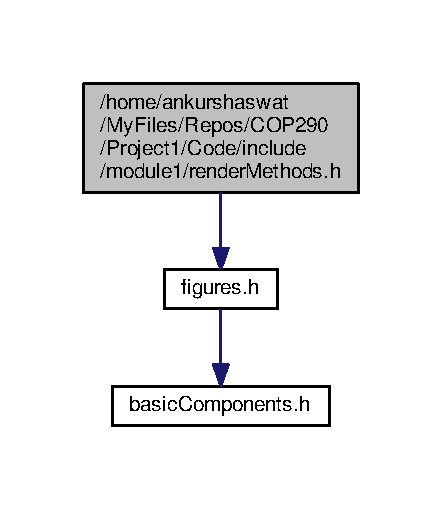
\includegraphics[width=318pt]{renderMethods_8h__incl}
\end{center}
\end{figure}
This graph shows which files directly or indirectly include this file\+:
\nopagebreak
\begin{figure}[H]
\begin{center}
\leavevmode
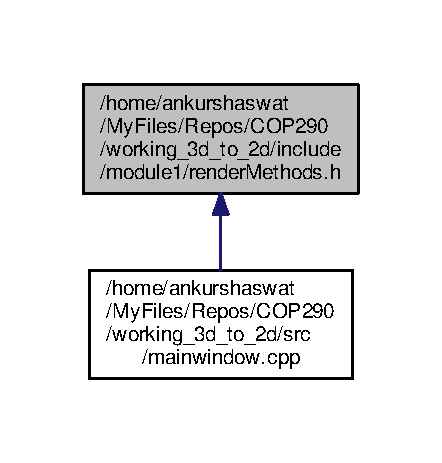
\includegraphics[width=217pt]{renderMethods_8h__dep__incl}
\end{center}
\end{figure}
\subsection*{Functions}
\begin{DoxyCompactItemize}
\item 
void \hyperlink{renderMethods_8h_ab6043f874ec8d70f6af6449bbf1ab02a}{render} (\hyperlink{classFig3D}{Fig3D} a)
\begin{DoxyCompactList}\small\item\em Function to render a 3d figure. \end{DoxyCompactList}\item 
void \hyperlink{renderMethods_8h_abbe049f22c313df9c0fe89db2a69f154}{render2D} (\hyperlink{classFig3D}{Fig3D} \&object3D, Q\+Painter \&painter, int plane)
\begin{DoxyCompactList}\small\item\em Function to render 2d views generated from 3d object. \end{DoxyCompactList}\item 
void \hyperlink{renderMethods_8h_a75faaca4675cd8cd28ae49e79c140c42}{render\+Axes} (\hyperlink{classFig3D}{Fig3D} \&object3D, Q\+Painter \&painter, int plane, double scale\+\_\+factor)
\begin{DoxyCompactList}\small\item\em Function to display axes on the labels for reference. \end{DoxyCompactList}\end{DoxyCompactItemize}


\subsection{Function Documentation}
\mbox{\Hypertarget{renderMethods_8h_ab6043f874ec8d70f6af6449bbf1ab02a}\label{renderMethods_8h_ab6043f874ec8d70f6af6449bbf1ab02a}} 
\index{render\+Methods.\+h@{render\+Methods.\+h}!render@{render}}
\index{render@{render}!render\+Methods.\+h@{render\+Methods.\+h}}
\subsubsection{\texorpdfstring{render()}{render()}}
{\footnotesize\ttfamily void render (\begin{DoxyParamCaption}\item[{\hyperlink{classFig3D}{Fig3D}}]{a }\end{DoxyParamCaption})}



Function to render a 3d figure. 

Methods for rendering 3D object and diplaying 2D views (will use Open\+GL and G\+TK libraries) \mbox{\Hypertarget{renderMethods_8h_abbe049f22c313df9c0fe89db2a69f154}\label{renderMethods_8h_abbe049f22c313df9c0fe89db2a69f154}} 
\index{render\+Methods.\+h@{render\+Methods.\+h}!render2D@{render2D}}
\index{render2D@{render2D}!render\+Methods.\+h@{render\+Methods.\+h}}
\subsubsection{\texorpdfstring{render2\+D()}{render2D()}}
{\footnotesize\ttfamily void render2D (\begin{DoxyParamCaption}\item[{\hyperlink{classFig3D}{Fig3D} \&}]{object3D,  }\item[{Q\+Painter \&}]{painter,  }\item[{int}]{plane }\end{DoxyParamCaption})}



Function to render 2d views generated from 3d object. 

\mbox{\Hypertarget{renderMethods_8h_a75faaca4675cd8cd28ae49e79c140c42}\label{renderMethods_8h_a75faaca4675cd8cd28ae49e79c140c42}} 
\index{render\+Methods.\+h@{render\+Methods.\+h}!render\+Axes@{render\+Axes}}
\index{render\+Axes@{render\+Axes}!render\+Methods.\+h@{render\+Methods.\+h}}
\subsubsection{\texorpdfstring{render\+Axes()}{renderAxes()}}
{\footnotesize\ttfamily void render\+Axes (\begin{DoxyParamCaption}\item[{\hyperlink{classFig3D}{Fig3D} \&}]{object3D,  }\item[{Q\+Painter \&}]{painter,  }\item[{int}]{plane,  }\item[{double}]{scale\+\_\+factor }\end{DoxyParamCaption})}



Function to display axes on the labels for reference. 


\hypertarget{structs_8h}{}\section{/home/ankurshaswat/\+My\+Files/\+Repos/\+C\+O\+P290/working\+\_\+3d\+\_\+to\+\_\+2d/include/module1/structs.h File Reference}
\label{structs_8h}\index{/home/ankurshaswat/\+My\+Files/\+Repos/\+C\+O\+P290/working\+\_\+3d\+\_\+to\+\_\+2d/include/module1/structs.\+h@{/home/ankurshaswat/\+My\+Files/\+Repos/\+C\+O\+P290/working\+\_\+3d\+\_\+to\+\_\+2d/include/module1/structs.\+h}}
This graph shows which files directly or indirectly include this file\+:
\nopagebreak
\begin{figure}[H]
\begin{center}
\leavevmode
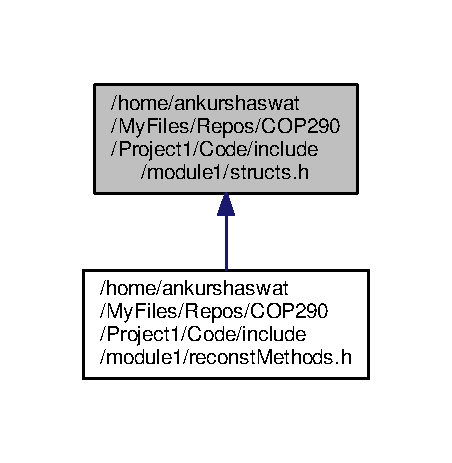
\includegraphics[width=350pt]{structs_8h__dep__incl}
\end{center}
\end{figure}
\subsection*{Classes}
\begin{DoxyCompactItemize}
\item 
class \hyperlink{classpartialOrder}{partial\+Order}
\end{DoxyCompactItemize}

\hypertarget{program_8cpp}{}\section{/home/ankurshaswat/\+My\+Files/\+Repos/\+C\+O\+P290/\+Project1/\+Code/src/program.cpp File Reference}
\label{program_8cpp}\index{/home/ankurshaswat/\+My\+Files/\+Repos/\+C\+O\+P290/\+Project1/\+Code/src/program.\+cpp@{/home/ankurshaswat/\+My\+Files/\+Repos/\+C\+O\+P290/\+Project1/\+Code/src/program.\+cpp}}


Main file documentation.  


{\ttfamily \#include $<$iostream$>$}\newline
Include dependency graph for program.\+cpp\+:\nopagebreak
\begin{figure}[H]
\begin{center}
\leavevmode
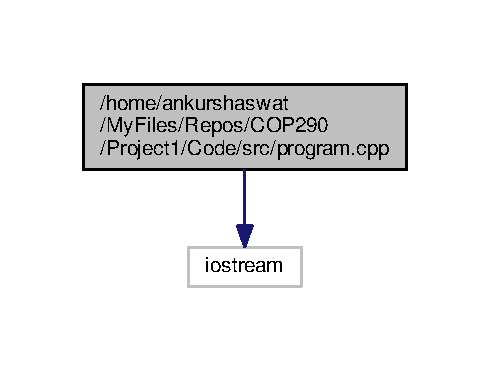
\includegraphics[width=235pt]{program_8cpp__incl}
\end{center}
\end{figure}
\subsection*{Functions}
\begin{DoxyCompactItemize}
\item 
int \hyperlink{program_8cpp_ae66f6b31b5ad750f1fe042a706a4e3d4}{main} ()
\end{DoxyCompactItemize}


\subsection{Detailed Description}
Main file documentation. 

\begin{DoxyAuthor}{Author}
Lastname\+:\+Firstname\+:\+A00123456\+:cscxxxxx 
\end{DoxyAuthor}
\begin{DoxyVersion}{Version}
Revision 1.\+0
\end{DoxyVersion}
Main File \begin{DoxyDate}{Date}
Monday, March 5, 2018 
\end{DoxyDate}


\subsection{Function Documentation}
\mbox{\Hypertarget{program_8cpp_ae66f6b31b5ad750f1fe042a706a4e3d4}\label{program_8cpp_ae66f6b31b5ad750f1fe042a706a4e3d4}} 
\index{program.\+cpp@{program.\+cpp}!main@{main}}
\index{main@{main}!program.\+cpp@{program.\+cpp}}
\subsubsection{\texorpdfstring{main()}{main()}}
{\footnotesize\ttfamily int main (\begin{DoxyParamCaption}{ }\end{DoxyParamCaption})}


%--- End generated contents ---

% Index
\backmatter
\newpage
\phantomsection
\clearemptydoublepage
\addcontentsline{toc}{chapter}{Index}
\printindex

\end{document}
